\documentclass[12pt, letterpaper]{article}
\usepackage[utf8]{inputenc}
\usepackage{graphicx}
\usepackage{verbatim}
\graphicspath{ {/home/xavfun/repos/gesture-processing-figures} }
\usepackage{amsmath}
\usepackage{geometry}

\title{Programmatic Visualization of Scientific Data and Study Designs for Neuroimaging}
\author{Xaver Funk}
\date{\today}

% write code
%(\verb!x_out!)

%https://acclab.github.io/DABEST-python-docs/robust-beautiful.html
\begin{document}
\maketitle
\section{Introduction}

Scientific publications rely heavily on graphical visualizations for communicating study designs, results and statistical outcomes. % sth generally about visualization in science

%[Data visualization is] the rendering of information in a visual format to help communicate data while also generating new patterns and knowledge through the act of visualization itself

For neuroimaging specifically, visualization plays an important role for a variety of reasons: 
For neuroimaging specifically, visualization plays an important role in a variety of challenges:


Firstly, neuroimaging studies often employ a generalizable framework for statistical analysis, namely the Generalized Linear Model (GLM). This allows any given study to construct an idiosyncratic set of regressors of interest and confound regressors to explain the data. Their construction reflects a central part of experimental design that has been a source of increasing complexity, especially in the light of event-related designs and naturalistic stimuli. Consequently, the visualization of regressor design as a means of communicating both the experimental and statistical setup has becone an indispensable tool for researchers in the field.

Secondly, as the name implies, neuroimaging is an inherently visual discipline. The endpoints of many studies show distributions of activity in the brain, whose localization, size and intensity are of crucial interest to the researchers. Essentially, communication of these characteristics of brain activity in a common reference space is heavily dependent on how they are visualized in a common reference space, such as the MNI template.

Lastly, when it comes to comparing different sets of datapoints, such as experimental groups or individual regressor's beta-values, classical statistical testing is increasingly supported by visualization of the data being compared. More traditional methods of displaying these comparisons do suffer from several drawbacks, with both bar- and boxplots possibly obscuring the sample size, as well as the true shape of a distribution underlying the data. While more transparent approaches, such as swarm- and violinplots are gaining popularity, parallel developments have yielded avenues to augment the displayed data by communicating additional comparative information. Thus, a growing toolkit enables researchers to more informatively and clearly visualize their data.

One such approach are Gardner-Altman plots, that display effect sizes as bootstrapped 95\% confidence intervals.  % put this maybe later

The current work is an exploration and hands-on implementation of data visualization approaches and tools that solve the aforementioned challenges in a real-world example. After giving a short introduction to the study and dataset considered here, this report is structured into... % recap the structure later

% mention, why python\programmatic

\section{the study at hand}
The study that builds the context for this work is a re-analysis of a previously published dataset, that the author worked on previoulsy during an fMRI practical course. Following, a concise of this study and analysis will be given, in order to set the context for the following visualizations. While in the MR-scanner, 20 paticipants were shown two videos of an actor narrating a short story while gesturing. With the consideration of multimodal sensory integration and a predictive-processing framework of language perception, a novel research question was conceived that ought to be answered using this data set: To what extent, if at all, does the processing of surprisal and entropy, two information-theoretic quantities implied in predictive processing, get facilitated through gestures?

During the aforementioned fMRI-practical, a set of regressors was constructed on a word-by-word basis that account for both the variables of interest, as well as possible confounds specific to the stimulus type. In order to answer the research question posed above, all content words of the story were split into two conditions, depending on whether a gesture was present or not. Consequently, one GLM was desinged for each of surprisal and entropy incorporating the different conditions and confound regressors. This allowed for the identification of several regions where.....



\section{Visualizing the study design}

\subsection{Rationale}
At hand is a study and analysis design with multimodal naturalistic stimulation employing two conditions investigated using a set of regressors containing one of two regressors of interest derived from information theory, two regressors based on confounding audiovisual information and one representing word frequency.
Due to the complexity inherent in this design, as well as the obscurity of some of the concepts involved, it is of central importance to communicate the relationships between stimuli, regressors and conditions in a concise manner. This challenge commonly presents itself to researchers when communicating sudy designs. 
Developed here is a graphical representation of these relationships that achieves this.

\subsection{Desiderata} % or challenges?
The following is a list of key desiderata that were identified and implemented in designing the visualization presented in figure \ref{fig:1}

\begin{enumerate}
	\item{relating the }


\end{enumerate}

\begin{verbatim}
test
\end{verbatim}


%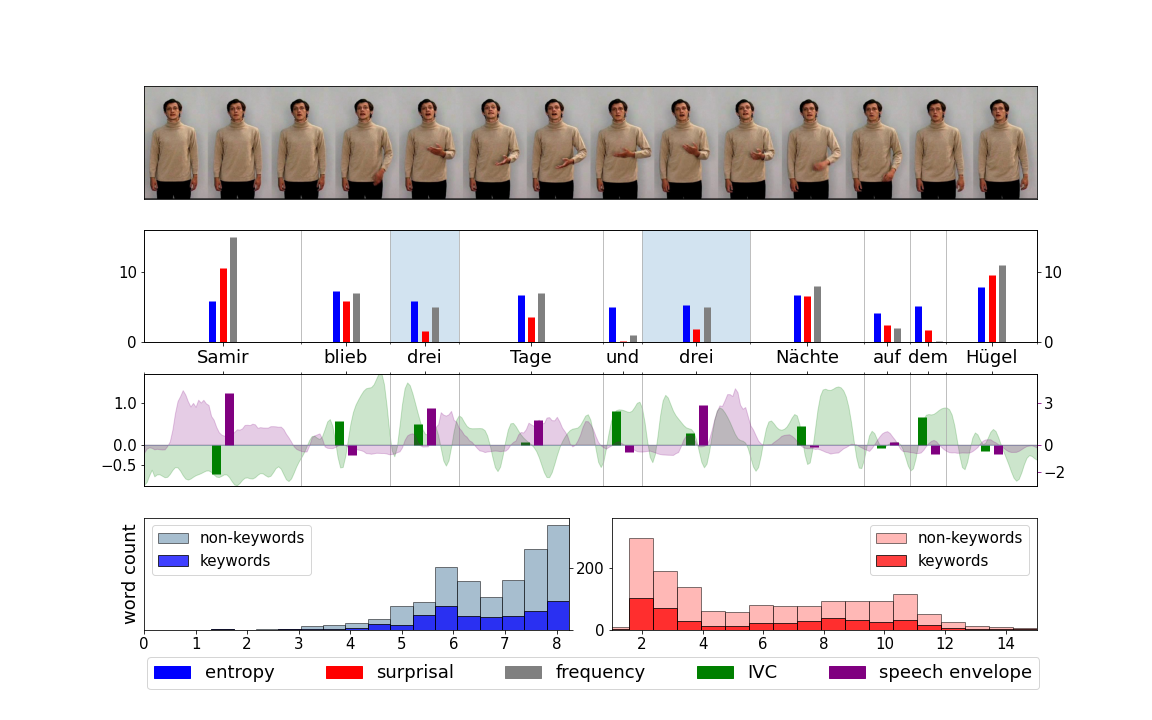
\includegraphics[scale=0.5]{figure1.png}
\begin{figure}
  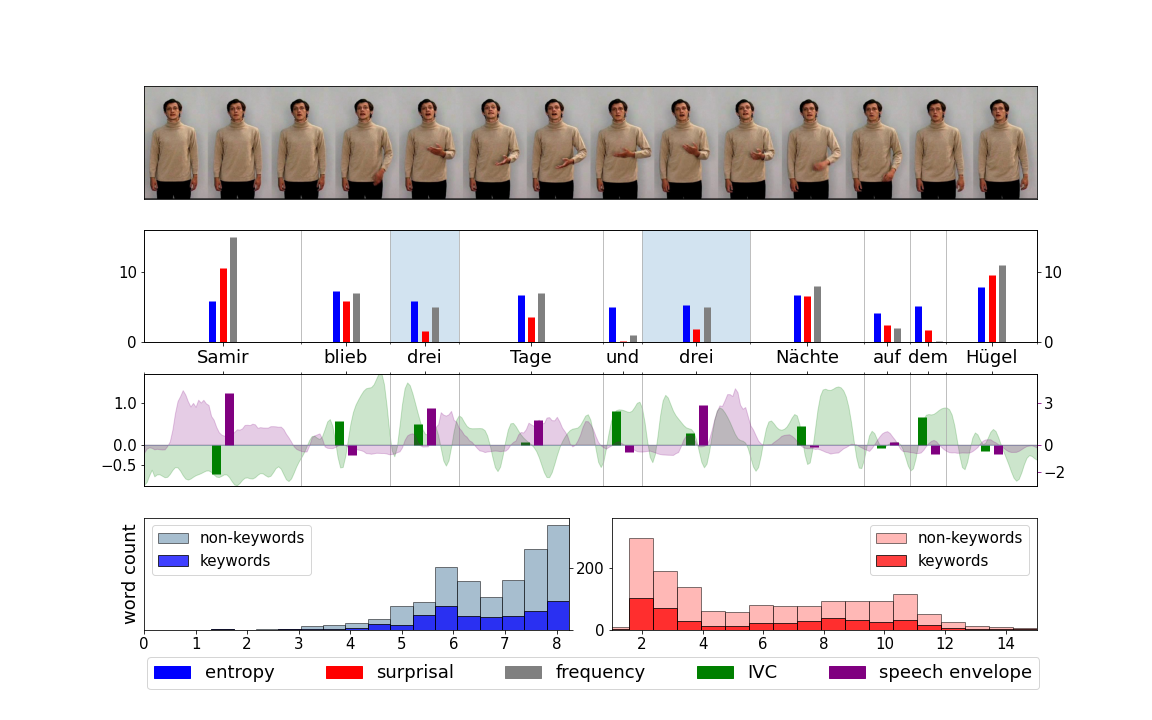
\includegraphics[width=\linewidth]{figure1.png}
  \caption{fig1}
  \label{fig:1}
\end{figure}

\section{Visualizing brain activations}

\subsection{Rationale}
As stated in the introduction, the extent and location of brain activations form an important endpoint for many kinds of neuroimaging studies.
Often, these kinds of visualization are done with software packages such as SPM and .. . 
However, since this work focuses on the programmatic implementation of visualizations, nilearn, a python library for brain imaging was used to develop the plot shown in figure 2.8422

\begin{figure}
  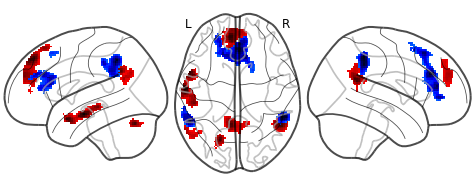
\includegraphics[width=\linewidth]{Figure2.png}
  \caption{fig2}
  \label{fig:1}
\end{figure}


\section{Visualizing condition comparison}

\subsection{Rationale}
Common approaches to comparing groups suffer from different shortcomings: bar plots hide the underling shape of the distribution and boxplots fail to convey sample size. 
However, there are tools available that solve these issues, such as swarm- and violinplots. 
Furthermore, when comparing groups or conditions, additional information can be incorporated in the plot, such as 95 \% confidence intervals on effects size or summary statistics, such as mean and standard deviation.
This chapter exemplifies the use of such advanced visualization tools using region-wise beta values derived from the GLM as a test case.

\begin{figure}
  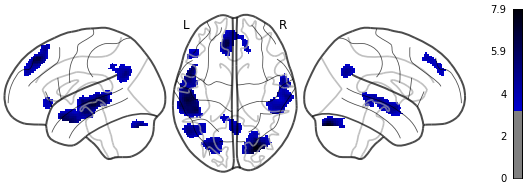
\includegraphics[width=\linewidth]{Figure3A.png}
  \caption{fig3}
  \label{fig:1}
\end{figure}


% add a disclosure explaining how this came to be, with time estimates of how much work put in etc
% maybe do it in the beginning
\end{document}





